\section{Hintergrund}
\label{sec-2}
\begin{comment}
\begin{center}
\fbox{
\parbox{0.9\linewidth}{
\textit{Ziel des Kapitels:}\\
Hintergründe der Arbeit in 3 Abschnitten: HoloLens Technik, AR in Education und Physik Hintergründe.\\
}}\\
\end{center}
\end{comment}
TODO: Einleitender Satz zu den Hintergründen der Arbeit

\subsection{HoloLens}
\label{sec-2-1}
\begin{comment}
\begin{center}
\fbox{
\parbox{0.9\linewidth}{
\textit{Ziel des Kapitels:}\\
HoloLens und Mixed Reality Toolkit mit ihrer Technik und Interaktionsweise vorstellen.
}}
\end{center}
\end{comment}

\subsubsection{Mixed und Augmented Reality}
\label{sec-2-1-1}

\begin{figure}[h!]
	\centering
	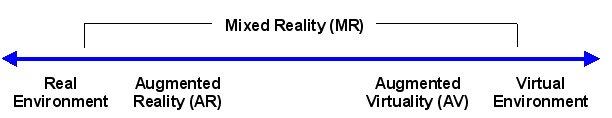
\includegraphics[width=0.9\textwidth]{images/papers/virtual_continuum.png}
	\caption{Virtual Continuum eingeführt von Paul Milgram \cite{Milgram94}}
	\label{img:virtual_continuum}
\end{figure}

Der Begriff \textit{Mixed Reality} (MR) wurde von Paul Milgram und Fumio Kishino in deren Arbeit \textit{``A Taxonomy of Mixed Reality Visual Displays''} im Jahr 1994 eingeführt \cite{Milgram94}. Die Autoren stellen das Konzept eines \textit{Virtual Continuums} vor, einem kontinuierlichen Spektrum zwischen vollständig realer und vollständig virtueller Umgebung. Augmented Reality findet sich damit auf der linken Seite des Spektrums wieder, dem entgegen steht Augmented Virtuality auf der rechten Seite. Als Mixed Reality wird der gesamte Bereich des Continuums bezeichnet, der zwischen den beiden Extremen ``völlig real'' und ``völlig virtuell'' liegt. Schema \ref{img:virtual_continuum} skizziert diesen Zusammenhang.\\

\begin{comment}
An dieser Stelle sei erwähnt, dass sich auch andere Interpretationen des MR-Begriffes finden. So beschreibt Jon Peddie MR als Kombination von realer und virtueller Welt, bei der beide co-existieren, wobei die MR Anwendung Informationen über die Umgebung und darin vorhandene Objekte nutzt \cite{Peddie17}. MR wird also eher als Erweiterung von AR verstanden, als eine übergeordnete Kategorie. Diese Herangehensweise findet sich auch bei manchen Internetquellen\footnote{https://www.intel.de/content/www/de/de/tech-tips-and-tricks/virtual-reality-vs-augmented-reality.html} \footnote{https://www.forbes.com/sites/quora/2018/02/02/the-difference-between-virtual-reality-augmented-reality-and-mixed-reality}.\\
\end{comment}

Beim Begriff der \textit{Augmented Reality} (AR), der ebenfalls kurz definiert werden soll, folgt diese Arbeit der gängigen Definition von Ronald T. Azuma \cite{Azuma97}. Dabei werden unter AR Techniken zusammengefasst, die es dem Nutzer erlauben, die reale Welt zu sehen, welche überlagerte oder eingebettete virtuelle Objekte enthält. Dafür hat eine Technik drei Charakteristiken aufzuweisen, sie:
\begin{enumerate}
	\setlength{\itemsep}{-5pt}
	\item Kombiniert reales und virtuelles
	\item Ist interaktiv (in Echtzeit)
	\item Steht in einem dreidimensionalen, räumlichen Zusammenhang
\end{enumerate}

\begin{comment}
Entsprechend der zuvor angesprochenen Variationen im Verständnis von Mixed Reality gibt es Diskussionen darüber, wie die HoloLens zu klassifizieren ist. Microsoft selbst ordnet sie als MR Gerät ein. Andere argumentieren, die Möglichkeiten der Brille seinen mit dem Begriff der Augmented Reality bereits abgedeckt. Peddie beispielsweise schreibt, dass ``Microsoft jedoch, möglicherweise aus Gründen des Marketing und der besseren Produktabgrenzung, darauf besteht, sie sei als MR Device einzuordnen'' \footnote{Zitat frei aus dem Englischen übersetzt.} \cite{Peddie17}.\\

Da diese Arbeit sich am MR Begriff von Milgram orientiert und mit der HoloLens unterschiedlich stark immersive Anwendungen möglich sich, wird die HoloLens im Folgenden allgemein als MR Device bezeichnet.

% TODO Ggf. Beispiele für AR/MR ANwendungen anführen
\end{comment}

Die HoloLens deckt mit ihren technischen Möglichkeiten vor allem den linken Bereich des Spektrums ab. Viele Anwendungen liegen deshalb im Teilbereich Augmented Reality.

Die HoloLens ist ein von Microsoft entwickeltes \textit{Head-Mounted Display} (HMD), das seit 2016 auf dem Markt ist. Das Gerät ist in der Lage, virtuelle Darstellungen in der Umgebung des Trägers zu verankern und anzuzeigen. Abbildung \ref{img:hololens} zeigt die Brille in der Standardausführung. Die technischen Eigenschaften und genutzten Techniken des HMDs bringen verschiedene Implikationen und Einschränkungen für Anwendungen auf der HoloLens mit sich. Daher soll im Folgenden auf die technischen Aspekte näher eingegangen werden.\\

\begin{figure}[h!]
	\centering
	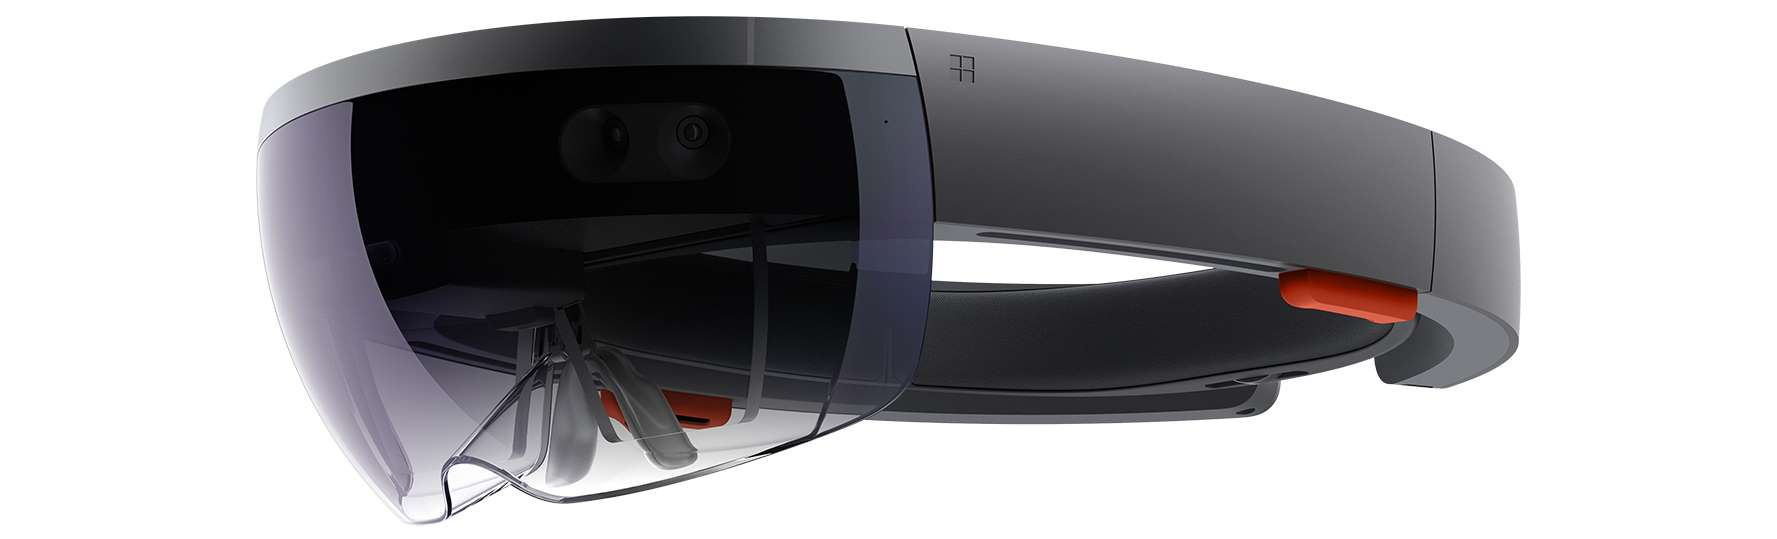
\includegraphics[width=0.9\textwidth]{images/papers/hololens.jpg}
	\caption{Die HoloLens in der Developer Edition (Quelle: Microsoft)}
	%https://www.microsoft.com/de-de/hololens
	\label{img:hololens}
\end{figure}

\subsubsection{Die Hardware}
Bei dem Device handelt es sich um einen eigenständigen Computer, auf dem eine spezielle Version von Windows 10 läuft. Die Brille arbeitet also völlig autonom und ist nicht auf externe Hardware wie z.B. zusätzliche Rechen- und Batterieeinheiten angewiesen.\\

\label{sec-2-1-2}
\begin{figure}[h!]
	\centering
	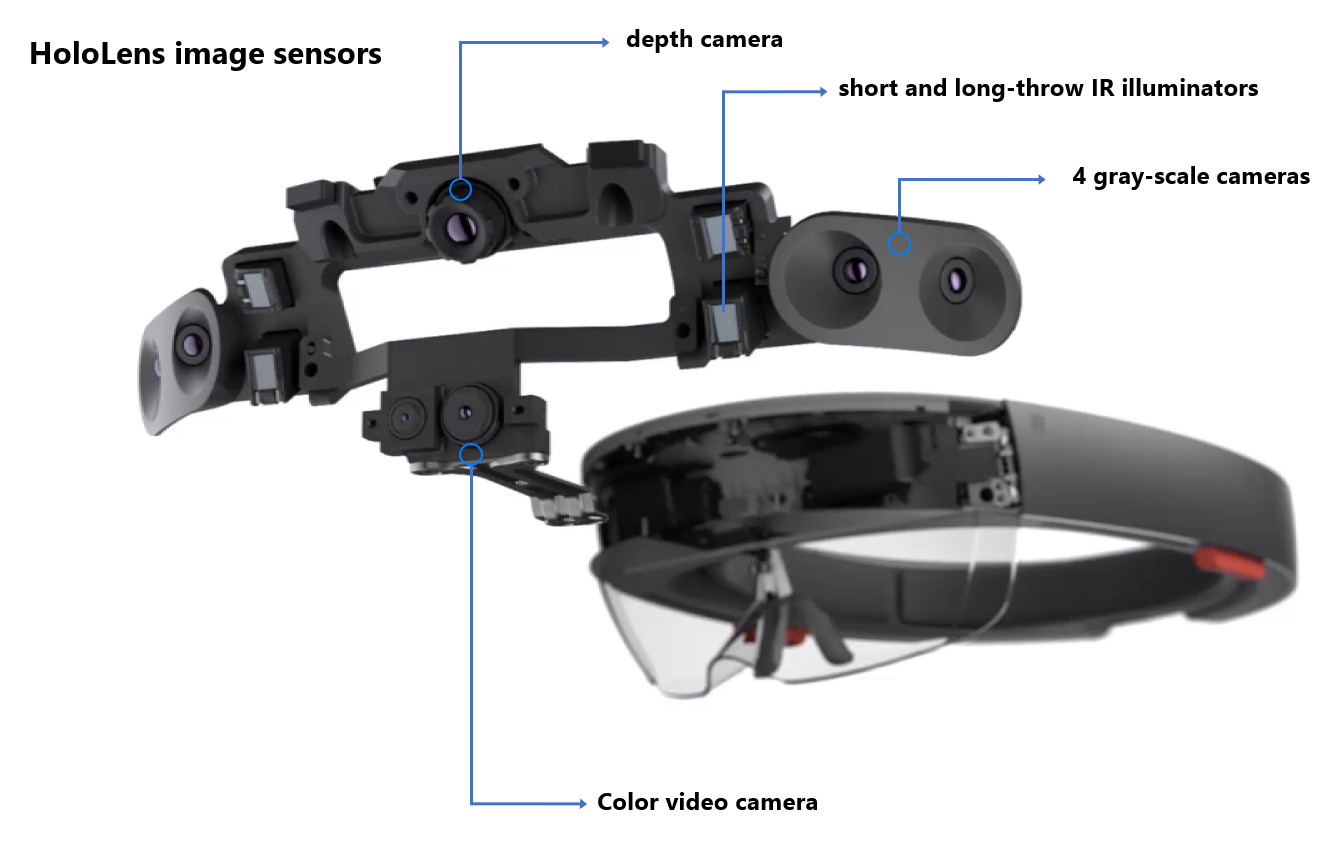
\includegraphics[width=0.9\textwidth]{images/papers/hololens_tech.png}
	\caption{Die Sensorik der HoloLens (Quelle: Microsoft)}
	%https://docs.microsoft.com/en-us/windows/mixed-reality/hololens-hardware-details
	\label{img:hololens_tech}
\end{figure}

Einen Überblick über die verwendete Hardware gibt Tabelle \ref{tab:hololens_tech_details}.

\bgroup
\setlength\extrarowheight{0pt}
\def\arraystretch{1.25}
\begin{table}[H]
	\centering
	\begin{tabular}{l|l}
		Kategorie & Eigenschaft\\
		\hline
		\hline
		Anzeige & 720p (HD) in 16:9 Format pro Auge\\
		& 60 Hz Bildwiederholrate\\
		& Blickfeld ca. 32°\\
		\hline
		Prozessor & Intel 32-Bit Prozessor @ 1.0 GHz\\
		\hline
		Grafik & Microsoft Holographic Processing Unit (HPU)\\
		\hline
		Arbeitsspeicher & 2 GB RAM\\
		& 1 GB HPU RAM\\
		\hline
		Speicher & 64 GB Flash Speicher\\
		\hline
		Kamera & 2 MP Foto / HD Video Front-Kamera\\
		\hline
		Sensoren & Inertiale Messeinheit (Accelerometer, Gyroskop, Magnetometer) \\
		& Zwei Stereo Kameras\\
		& 120° x 120° Tiefenkamera\\
		& Vier Mikrofone\\
		& Ambient Light Sensor\\
		\hline
		Akku & 2-3h Akkulaufzeit \\
		\hline
		Gewicht & 579 Gramm \\
		\hline
		Konnektivität & WiFi, BLE, USB 2.0, 3.5 mm Audio Jack \\
		\hline
		Audio & Lautsprecher mit Raumklang-Unterstützung\\
		\hline
		Steuerung & Gestensteuerung\\
		& Sprachsteuerung\\
		& HoloLens Klicker, Controller, Maus, Tastatur\\
	\end{tabular}\caption{\label{tab:hololens_tech_details} Spezifikation der HoloLens. Quelle: Microsoft}
\end{table}
\egroup

\vspace{4px}
\textit{Das Display}\\
Kernstück des Gerätes ist das durchsichtige, stereoskopische Display, mit dem die virtuellen 3D-Objekte angezeigt werden. Durchsichtig bedeutet, dass das Display für Licht von außen durchlässig ist und der Nutzer somit wie durch eine Brille seine Umgebung sehen kann. Virtuelle Objekte werden zusätzlich dazu angezeigt, indem Licht über optische Wellenleiter (Optical Wave Guides) in das Display geleitet wird, welches das Licht dann auf die Augen reflektiert.\\

Anwendungen werden mit 60 Frames pro Sekunde dargestellt. Bei der Anzeige handelt es sich jedoch um ein \textit{Color Sequential Display}, bei dem die drei Farben Rot, Grün und Blau nacheinander dargestellt werden. Pro Bild werden folglich drei Einzelbilder (je eins pro Farbe) gezeigt, was eine Framerate von 240 Hz ergibt.\\

Es handelt sich dabei um ein stereoskopisches Display, bei dem pro Auge separat ein Bild dargestellt wird. So ermöglicht die HoloLens dem Träger das stereoskopische Wahrnehmen dreidimensionaler Objekte. Die beiden Bilder werden in einem festen Abstand von 22 mm zueinander dargestellt. Außerdem beträgt die Distanz, auf die sich die Augen einstellen müssen, damit Bilder als scharf wahrgenommen werden (Akkommodation), etwa zwei Meter und ist ebenfalls fest.\\

\vspace{4px}
\textit{Das Tracking}\\
Um die Hologramme im Raum verankern zu können, benötigt die HoloLens Informationen über ihre exakte Position und Orientierung im Raum. Beides erarbeitet das Gerät allein aus einem Zusammenspiel der verschiedenen internen Sensoren und ist nicht auf externe Markierungen angewiesen, es handelt sich um sogenanntes \textit{Inside-Out Tracking}. Das Vorgehen basiert dabei auf zwei Strategien.
\par
\noindent\hspace*{5mm}
Zum einen erfasst die HoloLens die Oberflächenstruktur der Umgebung über Tiefen- und Stereokameras. Während der Nutzer sich durch den Raum bewegt, wird dies immer weiter vervollständigt und verbessert. Dieses Vorgehen wird \textit{Spatial Mapping} genannt und kann auch von Anwendungen genutzt werden, um mit Objekten der realen Welt zu interagieren.
\par
\noindent\hspace*{5mm}
Zum anderen kommt eine inertiale Messeinheit zum Einsatz. Über die Beschleunigungs-, Rotations- und Magnetflusssensoren können Änderungen in Position und Ausrichtung der Brille gemessen werden. Bei diesem Vorgehen summieren sich Messfehler im Laufe der Zeit jedoch stetig weiter auf und die Positionsschätzung wird zunehmend unzuverlässiger. Daher wird ein Zusammenspiel mit der Raumerkennung genutzt.

\begin{comment}
 Das Vorgehen lässt sich dabei in zwei Bereiche unterteilen:
 Als Grundlage dazu dienen zum einen eine Tiefenkamera, die anhand der Time-of-Flight von ausgestrahltem Infrarotlicht die Entfernung zu nahegelegenen Oberflächen, die das Licht reflektieren, bestimmt. Zum anderen unterstützen die beiden Stereo-Kameras diese Informationen durch Triangulation von Objekten. Auf diese Weise erarbeitet die Brille ein 3D-Gitternetz, das nach und nach aktualisiert und vervollständigt wird, wenn sich der Träger im Raum bewegt. Anhand dieses sogenannten \textit{Spatial Mapping} wird ein Ankerpunkt für ein im Raum festes Koordinatensystem ausgewählt, dass der Brille als Referenzsystem dient.\\


Um die exakte Position und Ausrichtung der HoloLens nachzuverfolgen kommt außerdem die inertiale Messeinheit zum Einsatz. Die Beschleunigungs-, Rotations- und Magnetflusssensoren ermöglichen Schlussfolgerungen zu Änderungen in Position und Orientierung über eine Zeitdifferenz. Zusammen mit den Informationen aus den optischen Verfahren leitet die Brille so ihre genaue Position und Ausrichtung ab. Darüber hinaus speichert und unterscheidet das Gerät verschiedene Räume anhand der unterschiedlichen Struktur und den dort vorhandenen WLAN Signalen.\\
\end{comment}

\subsubsection{Die Software und Interaktion}
\label{sec-2-1-3}
Auf der HoloLens läuft eine spezielle Version von Windows 10. Diese benötigt weniger Resourcen im Vergleich zu einem herkömmlichen PC und hat daher auch einen eingeschränkten Funktionsumfang. Anwendungen werden in Form von UWP Apps bereitgestellt. Hier unterstützt Microsoft die Entwicklung mit Unity und stellt entsprechende Toolkits zur Verfügung.\\

Die Steuerung durch den Nutzer erfolgt auf vier verschiedene Arten:
\begin{itemize}[topsep=-2px]
	\setlength{\itemsep}{-1pt}
	\singlespacing
	\item Blickrichtung (Orientierung des Kopfes)
	\item Handgesten
	\item Sprachbefehle
	\item Externe Eingabegeräte (Controller, Maus, Tastatur, etc.)
\end{itemize}
\vspace{6px}

Handgesten werden von der HoloLens automatisch erkannt und an die Anwendung in Form von Events weitergegeben, auf welche dann reagiert werden kann. Hier sind aktuell verschiedene Klick-Gesten zu nennen, durch die bekannte Mausfunktionen wie Klick, Click-and-Hold, Doppelklick und Drag-and-Drop abgebildet werden. Der Cursor orientiert sich dabei an der aktuellen Blickrichtung: Es wird automatisch das Objekt angeklickt, das als erstes von einer zentralen, vorwärts gerichteten Linie getroffen würde. Außerdem gibt es eine spezifische Handgeste zum aufrufen des Hauptmenüs.\\

Darüber hinaus nimmt die HoloLens englische Wörter als Sprachbefehle an, die sich auch kombinieren lassen. So kann eine Anwendung die Phrase ''Hello World'' als Keyword registrieren und dann darauf reagieren. Über Bluetooth lassen sich weitere Eingabegeräte anschließen: Den mit der HoloLens mitgelieferten Klicker, der die Klick-Geste ersetzen kann, aber auch eine Tastatur oder ein Controller lassen sich nutzen.\\

\vspace{4px}
\textit{Das Mixed Reality Toolkit}\\
Das \textit{Mixed Reality Toolkit} (MRTK) ist ein quelloffenes Toolkit, das elementare Funktionen für die Entwicklung von Mixed Reality Anwendungen, insbesondere auch für die HoloLens, bereitstellt. Dazu gehört beispielsweise ein Objekt, das den zuvor genannten Cursor implementiert, aber auch Funktionen, die das Spatial Mapping auswerten. Für die Entwicklung mit Unity gibt es das Toolkit als Unitypackage, das unter anderem folgende Features bereitstellt:

\begin{itemize}[topsep=-2px]
	\setlength{\itemsep}{-1pt}
	\singlespacing
	\item Kameraobjekt mit den korrekten Einstellungen für die HoloLens
	\item Stabilisiertes Cursorobjekt mit Animationen für verschiedene Klicks
	\item Manager-Objekte, die Steuerung von Inputs und des Spatial Mappings erlauben
	\item Skripte für Standard Interaktionen wie Drag-and-Drop und Skalierung
	\item Für HoloLens angepasste Materialien und Shader
	\item Vorgefertigte und anpassbare UI-Elemente wie Buttons, Tooltips, Icons und Dialoge
\end{itemize}
\vspace{6px}

Für die Entwicklung mit dem Toolkit und der HoloLens existiert ein umfassendes Repertoire aus Dokumentation, Beispielen, Guidelines, Einführungen und Hinweisen.\\


\subsubsection{Implikationen für Anwendungsdesign}
\label{sec-2-1-4}
Die technischen Eigenschaften der HoloLens haben Auswirkung auf Design und Nutzung von Anwendungen. Dazu gehören auch technisch bedingte Einschränkungen sowie zu berücksichtigende Aspekte für die Usability und Nutzererfahrung. Im Folgenden soll auf ausgewählte solcher Zusammenhänge hingewiesen werden.\\

\textit{Tracking}\\
Ein wichtiger Punkt ist, das Tracking nicht zu behindern, da die Darstellungen andernfalls nicht korrekt im Raum positioniert werden können. Für die Stereo- und Tiefenkamera sind sehr dunkle und transparente Materialien problematisch, da hier kaum (Infrarot-) Licht reflektiert wird und so entsprechende Gegenstände nicht erkannt werden. Spiegelnde Materialien sind daher ebenfalls ungünstig.\\

\textit{Display}\\
Die Displays sind, vergleichbar mit einem Beamer, in der Lage den Hintergrund zu überblenden, nicht jedoch ihn abzudunkeln. Dementsprechend ist kein Schwarz darstellbar. Wie transparent Objekte auf der HoloLens erscheinen, hängt folglich auch vom Hintergrund und der Umgebungshelligkeit ab. Ein sehr heller Hintergrund kann von der HoloLens nicht vollständig überblendet werden.
\par
\noindent\hspace*{5mm}
Außerdem hängt die Transparenz virtueller Objekten von ihrer Farbe ab. Ein blauer Pixel leuchtet nur in jedem dritten Frame auf, ein weißer hingegen in jedem Frame, da die Farben sequentiell dargestellt werden.\\

Bedingt durch die Displaytechnik wirken Objekte scharf, wenn sich die Augen auf eine Distanz von zwei Metern einstellen (Akkommodation). Die Augen sind jedoch daran gewöhnt, dass nah liegende Objekte eine andere Akkommodation erfordern, als weiter entfernte. Dies kann vor allem bei sehr dicht liegenden Objekten dazu führen, dass Nutzer sich unwohl fühlen oder die Objekte nicht richtig erkennen können.

%TODO
\begin{minipage}{0.48\textwidth}
	\centering
	\includegraphics[width=0.9\textwidth]{images/todo.jpg}
	\label{img:acco-convergence}
\end{minipage}\begin{minipage}{0.48\textwidth}
	\centering
	\includegraphics[width=0.9\textwidth]{images/todo.jpg}
\end{minipage}\\

\par
\noindent\hspace*{5mm}
Im Zusammenhang der Akkommodation spielt hier auch die Konvergenz der Augen eine Rolle. Darunter versteht man die Bewegung der Augen aufeinander zu, sodass der Punkt, in dem sich die Gesichtslinien treffen, näher kommt. Eine Illustration des Zusammenhangs bietet Abbildung \ref{img:acco-convergence}. Dieser Vorgang ist wichtig, damit Objekte nicht doppelt gesehen werden. Akkommodation und Konvergenz sind auf natürliche Weise gekoppelt: Um ein dicht liegendes Objekt zu betrachten laufen die Augen weiter zusammen und erhöhen ihre Brechkraft. Dieser Effekt wird auch Akkommodation-Konvergenz-Reflex genannt. Beim Tragen der HoloLens kann es jedoch dazu kommen, dass dieses Zusammenspiel aufgebrochen wird.
\par
\noindent\hspace*{5mm}
Angenommen ein Nutzer fokussiert ein reales Objekt in einer Entfernung unter zwei Metern. Jetzt wird ein virtuelles Objekt räumlich vor dem realen Objekt positioniert. Jetzt müssen Akkommodation und Konvergenz gegenläufig arbeiten: Die Augen müssen sich aufeinander zu bewegen, die Brechkraft dabei jedoch abnehmen, da sie sich auf zwei Meter anpassen muss. Dies steht im Gegensatz zum Akkommodation-Konvergenz-Reflex und kann die Nutzererfahrung negativ beeinflussen.\\

Sowohl für Akkommodation als auch Konvergenz gilt jedoch, dass die Unterschiede mit zunehmender Distanz kleiner werden und die Probleme deshalb vor allem bei kurzen Distanzen auftreten.\\

\textit{Hardwareressourcen}\\
Die Hardwareressourcen der HoloLens sind mit einer CPU und GPU mit jeweils 1 GHz und 1GB RAM stark limitiert. Anwendungen sollten daher möglichst ressourcenschonend sein. Auf rechenintensive Operationen wie z.B. Schattenberechnungen oder Kantenglättung muss meist verzichtet werden.\\

\textit{Framerate}\\
Dabei ist es von besonderer Bedeutung, dass die Anwendung möglichst konstant 60 Bilder pro Sekunde ausgibt. Um die Hologramme im Raum stabil und ohne Ruckler oder Zittern anzuzeigen, müssen selbst feinste Kopfbewegungen ausgeglichen werden. Dazu nutzt die HoloLens ein spezielles Verfahren:
\par
\noindent\hspace*{5mm}
Bevor eine Szene in die Render-Pipeline geht, trifft die Brille anhand der Sensordaten eine Vorhersage darüber, in welcher Position und Ausrichtung sich die Brille befinden wird, wenn das zu errechnende Bild dargestellt wird. Anhand dieser Schätzung wird die Kamera-Position und -Ausrichtung für die Szene festgelegt und anschließend gerendert. Eine längere oder variierende Renderzeit bedeutet damit auch eine unzuverlässigere Schätzung. Das kann zu instabil wirkenden Darstellungen führen, z.B. in Form von Zittern oder Ruckeln. Deshalb empfiehlt Microsoft, die Framerate von 60 FPS stets aufrecht zu erhalten.\\

\subsubsection{Empfehlungen zu Design und Umsetzung}
\label{sec-2-1-5}
Damit Einschränkungen umgangen und negative Auswirkungen vermieden werden können, gibt es bereits einige Designempfehlungen und Guide-Lines sowie Empfehlungen zur Implementierung. Die Dokumentation zu Windows Mixed Reality umfasst hier einige Vorschläge und Hinweise, von denen besonders relevante hier vorgestellt werden sollen.\\

\textit{Positionierung von Objekten}\\
Objekte sollten typischerweise aus einer Distanz zwischen einem und fünf Metern betrachtet werden, um die zuvor erläuterten Probleme mit der Wahrnehmung zu vermeiden. Deshalb sollten Objekte ausgeblendet werden, die zu nah kommen. Neben der Distanz spielt auch der Blickwinkel in der vertikalen eine Rolle. Damit ein Anwender die Darstellungen angenehm betrachten kann ist es wichtig, eine angenehme und natürliche Kopfposition zu ermöglichen. Hier wird ein Blickwinkel zwischen 0° und 35° unterhalb der Horizontlinie empfohlen.\\

Weiterhin ist die Größe von Objekten von Bedeutung. Das gilt besonders dann, wenn sie mit dem an die Kopfbewegungen gekoppelten Cursor anvisiert werden müssen. Zu kleine Objekte wären für den Anwender schwer zu treffen. Ein Winkel zwischen 1,5° und 3° des Sichtfeldes dienen hier als Orientierung. Allerdings sollten die Darstellungen auch nicht zu groß sein, da sie sonst schon bei geringen Kopfbewegungen durch die Begrenzung des Displays abgeschnitten werden.\\

Um Objekte wie z.B. Menus und Dialoge, die nicht fest im Raum verankert sind, anzupassen, stellt das Mixed Reality Toolkit verschiedene Funktionen wie z.B. Billboarding oder Tagalong zur Verfügung, die Abstand, Orientierung und Skalierung entsprechend der Nutzerbewegung automatisch anpassen.\\


TODO: Stabi Ebene und SPatial Anchors

\textit{Performance Optimierungen}\\
Da die Framerate maßgeblichen Einfluss auf die Stabilität von Hologrammen hat und die Hardwareressourcen limitiert sind, gibt es eine Reihe von empfohlenen Optimierungen und Hinweisen, um die Performance einer Anwendung zu verbessern. Diese umfassen unter anderem:
\begin{itemize}[topsep=-2px]
	\setlength{\itemsep}{-1pt}
	\singlespacing
	\item Singe Pass Instanced Rendering verwenden
	\item Z-Puffer Größe auf 16 Bit setzen
	\item Full-Screen Post Processing (z.B. FXAA) vermeiden
	\item Shader anpassen / vereinfachen
	\item Physics ausschalten
	\item Overdraw reduzieren
\end{itemize}
\vspace{6px}

Um die Performance bei der Entwicklung im Blick haben zu können gibt es einige Tools. Die HoloLens stellt über ein Webinterface einen Performance-Monitor zur Verfügung. Dieser gibt Auskunft über die Auslastung von Ressourcen wie CPU und GPU, ähnlich zum Windows Taskmanager. Außerdem verfügt Unity über einen Profiler, der detailliertere Informationen zum Renderingprozess liefert.\\

\textit{Weitere Empfehlungen}\\
Aus ihren Erfahrungen und dem Nutzerfeedback aus mehreren HoloLens-Applikationen geben Zimmer et. al. einige weitere Empfehlungen \cite{Zimmer17}. Im Folgenden ist eine Auswahl an für diese Arbeit besonders relevanten Aspekten zusammengefasst:
\begin{itemize}[topsep=-2px]
	\setlength{\itemsep}{-1pt}
	\singlespacing
	\item Einen sichtbaren Cursor in der Mitte des Blickfeldes für die Auswahl bzw. das Anklicken von Objekten nutzen
	\item Begrenzungen des Field-of-View (FOV) beachten: Wenn möglich Objektegröße so anpassen, dass diese ganz dargestellt werden können, da andernfalls Objekte weniger präsent wirken
	\item Die Einbettung von Objekten kann durch visuelle Anhaltspunkte wie Verdeckung oder Schatten unterstützt werden
	\item Spatial Mesh für grobe Verdeckung nutzbar, für genauere Verdeckung können reale Objekte nachmodelliert werden 
	\item Alternative Interaktionsmöglichkeiten (z.B. Klicker) können hilfreich sein, wenn Nutzer Probleme mit Gesten oder der Sprachsteuerung haben
	\item Eine Einführung in die Anwendung und insbesondere die Steuerung kann hilfreich sein, da der Umgang mit der HoloLens oder ähnlichen Geräten für Anwender meist ungewohnt ist
\end{itemize}
\vspace{6px}


